%!TEX root = ../../thesis.tex
\section{Differential Synchronization}
\label{sync-diffsync}

\begin{figure}[htb]
  \centerline{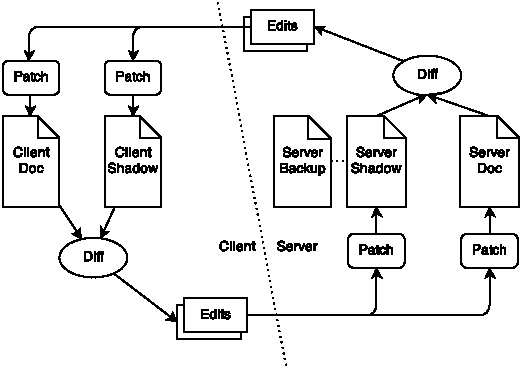
\includegraphics[width=0.8\linewidth]{images/Differential_Synchronization.pdf}}
  \caption[Illustration of Differential Synchronization - based upon
  \protect\newline{\small\url{https://neil.fraser.name/writing/sync/diff3a.gif} (02.5.2014)}
  \protect\newline{\small\emph{Neil Frasier}}]{Illustration of Differential Synchronization}
  \label{fig:DiffSync}
\end{figure}

Differential Synchronization (DS) is based on similar techniques that are also used in the Three-way merge algorithm (see: \refchapter{sync-3waymerges}). As a result of its highly different architecture, it is also suited for real-time collaborative editing. The algorithm, introduced by \cite{fraser2009differential},  has shown that it is stable and well-suited for interactive applications \cite[p. 8]{koren2013sharedediting}, despite the fact that it is a young algorithm in comparison to \refchapter{sync-ot}.

Server and client start off with an identical version of the document and then both create a copy of that document which will work as the shadow document of the client and as the shadow document of the server respectively. These shadows will always contain the state of the document that lies on the other end. As shown in \reffigure{fig:DiffSync}, the synchronization sequence is always initiated by a change of the document by a client. This change will trigger the creation of a diff between the local copy and the client shadow which is then added to the local stack of edits. A message that contains the newly created diff and metadata, such as checksums and version numbers, is built and sent to the server. The diff that is contained in the message is then patched to the server shadow (which represents the current state of the client) and the outcome is then compared to the checksum that was previously transmitted alongside the diff. If the checksum matches, the diff will also be applied to the server's copy of the document and the old version of the server shadow will be copied to the backup shadow. If the checksum does not match, the diff has been corrupted during transmission, which means the client needs to refetch the document and throw away the diff. Subsequent to patching the server's documents, a diff is created from the recently patched documents (shadow and server copy). This diff will include changes that were made to the document by other peers in the network. An edit message is created on the server and sent to the client, who then patches and diffes these changes again, in the same way as the server previously did.

The above process is restricted to one simultaneous request per user at one time in order to preserve consistency. Users are still permitted to edit the client's document during a request, but the changes will only be sent to the server after the last request been processed. In this way, DS ensures \textbf{Full Concurrency} and provides a mechanism of \textbf{Latency Hiding}.

DS is capable of handling packet losses for both requests and responses. By comparing version numbers of each edit on server and client and by keeping a stack of edits, the algorithm is able to detect and handle inconsistencies. If for example, a packet is lost on its way to the server, its edit will be sent the next time the client wants to send an update. This is because the client's edit-stack is only reset if it receives an edit from the server that contains the merge of the last edit. Since the server did not receive the last edit in this case, it did not send another edit to the client and the client's edits-stack is not emptied\footnote{\cite[p. 4]{fraser2009differential}}.

When a packet gets lost on its way to the client, the next client-request will contain incorrect version numbers and the server will load the backup shadow (which always represents the version before the last successful patch) into the server shadow. It will apply the edits to the backup document, because the version numbers will match this document. In this case, the server will need to throw away its edit stack, because the edits are now based on different versions, and will therefore only send a diff from the newly patched document.

A key factor of DS is the implementation of the diff and patch actions, which greatly depend on the underlying data structure. The diff implementation needs to have a high performance, because it could be executed several times a second, dependent on how often the client initializes a sync request. The patch implementation needs to be fuzzy, meaning it should be able to incorporate changes to documents that might have diverged over the course of several seconds. The fuzzy implementation should merge the diffs in way that it respects the semantics of the data structure. Diff and patch being the key factor of DS also means that it is agnostic to data structures. DS can be applied to all data structures that have adequate implementations of patch and diff\footnote{\cite[p. 5]{fraser2009differential}}. The combination of diff and patch is responsible for \textbf{Convergence} and \textbf{Intention Preservation} of the algorithm. The overall architecture of the technique ensures, that no document can reach a state where the causality of actions is violated, thus guaranteeing \textbf{causality preservation}\footnote{\cite[p. 1]{fraser2009differential}}.

The client should ensure that synchronization cycles are initiated more often than there are changes on the document. This is because a user may not edit the document for a while and in this time he will not receive updates from other collaborators due to the asynchronous nature of the initialization process. In addition to document changes, the synchronization process should get triggered at certain intervals to make the application seem more interactive \cite{instantSyncThesis}. The less time there is between synchronization cycles, the better will the diff and patch actions perform and the better will the algorithm perform in providing \textbf{graceful exit} methods. This is down to the fact that there will be smaller changes and therefore less contextual changes, which then leads to fewer conflicts in the document. This also implies that when a packet is corrupted during transmission, as described above, the system will lose only little information.

Although DS is based on a client-server architecture, it could also easily be adapted to make it usable in peer-to-peer networks. In this scenario all participants would be able to send their local changes to other peers, requiring each client to also have a backup document for every other peer in the network\footnote{\cite[39:20min]{fraser2009video}}. This makes the implementation of client and server even more analogue, since every client is now essentially a server in its own right.

% State transfer vs. operation transfer
% \cite{saito2005optimistic}